\documentclass[OPS,lsstdraft,authoryear,toc]{lsstdoc}
\input{meta}

% Package imports go here.

% Local commands go here.

%If you want glossaries
%\input{aglossary.tex}
%\makeglossaries

\title{Criteria to start the Legacy Survey of Space and Time}

% This can write metadata into the PDF.
% Update keywords and author information as necessary.
\hypersetup{
    pdftitle={Criteria to start the Legacy Survey of Space and Time},
    pdfauthor={First Last},
    pdfkeywords={}
}

% Optional subtitle
% \setDocSubtitle{A subtitle}

\author{%
Robert Blum, Charles F. Claver \v{Z}eljko Ivezi\'{c}, Phil Marshall
}

\setDocRef{RTN-093}
\setDocUpstreamLocation{\url{https://github.com/lsst/rtn-093}}

\date{\vcsDate}

% Optional: name of the document's curator
% \setDocCurator{The Curator of this Document}

\setDocAbstract{%
This document concisely captures the criteria that must be satisfied to begin regular survey operations for the Legacy Survey of Space and Time (i.e. to begin execution of the planned 10 year survey strategy currently documented in PSTN-056). It is expected that the survey will start in late 2025 1-2 months after the beginning of the formal Operations phase at the completion of construction. The survey can start based on quantitative criteria described herein. The system contribution to the delivered image quality must be $\ge$ 0.4$\arcsec$ and the effective survey speed must be 1.01 or better. Both of these are attainable given our experience and knowledge of the current on sky system. 
}

% Change history defined here.
% Order: oldest first.
% Fields: VERSION, DATE, DESCRIPTION, OWNER NAME.
% See LPM-51 for version number policy.
\setDocChangeRecord{%
  \addtohist{1}{2025-02-28}{01.0}{Robert Blum}
  \addtohist{1}{2025-09-01}{02.0 Criteria and Schedule updates}{Robert Blum}
}
\graphicspath{{./}{figures/}}
\usepackage{makecell}

\begin{document}

% Create the title page.
\maketitle
% Frequently for a technote we do not want a title page  uncomment this to remove the title page and changelog.
% use \mkshorttitle to remove the extra pages

% ADD CONTENT HERE
% You can also use the \input command to include several content files.

\section{Introduction}

By the end of October 2025 the Rubin Observatory will be substantially completed having passed its Construction Completeness Review \#3 (CCR3) and Operations Readiness Review \#2.  This will signify the formal handover of activities from the construction project to Rubin Operations. In practice, this means the Operations team \cite[see][]{RDO-018} will assume day-to-day responsibility of the Observatory and its regular operations: running the facility on Cerro Pach\'{o}n each night, transferring data over the long haul network to the US Data Facility (USDF), processing and archiving the data, and delivering data products to the user community via realtime alerts and scheduled data releases. 

At the time of handover the construction team will have demonstrated the overall Rubin Observatory system is \it{capable} of meeting its required science driven technical performance as articulated in the Science Requirements Document \cite{SRD}, LSST System Requirements \cite{LSR} and Observatory System Specifications \cite{OSS} documents.  It is expected that improvements to processes, sub-system reliability and performance consistency will be necessary in advance of formally beginning the execution of the the 10--year Legacy Survey of Space and Time (LSST). The survey strategy and it's associated cadence in the 10--year period (currently allowing for modest assumed degradation in year 1) are detailed by the Survey Cadence Optimization Committee \cite[SCOC,][]{PSTN-056}. 

In this technote, we define the set of key performance criteria that the Operations team, in consultation with operations partners -- the post-handover Construction team, the Rubin Management Board, funding agencies, and the science advisory committee -- will use to guide the decision to begin the LSST. 

The formal handover from construction to operations is scheduled to occur on October 25th, 2025. The primary science program for the Rubin Observatory -- the Legacy Survey of Space and Tinmme -- will begin after the handover to Operations and when the key ''start'' criteria have been met.  It is expected that the LSST will begin in ernest prior to the close of calendar year 2025.

Formal transition of construction staff into the Rubin Operations organization (derived jointly from NSF's NOIRLab under AURA and DOE's SLAC Rubin Operations) will be on October 1, 2025. See section~\ref{secSched} below for the current schedule.  

\section{System Performance}
  
Handover means that the system will have passed NSF and DOE close out review. The as delivered system will be capable of delivering images that satisfy the science requirements as defined in SRD (\cite{LPM-17}). Following the final phase of commissioning which will include science validation (SV) observations, the state of the system will be assessed and the readiness of the system and team to begin the survey will be made. 

Rubin has developed a high level metric to summarize the system performance with respect to survey efficiency. We need to ensure both that the system is producing science capable images and data products and that the observing is efficient. 
If the site and system are producing appropriate image quality and the system and team are acquiring data efficiently coming out of SV, we can confidently start the LSST. In Figure~\ref{fE}, we show the system contribution to image quality (and atmospheric contribution) versus the dimensionless survey efficiency or ``speed,'' fE. 

\begin{figure}%[!ht]
  \centering
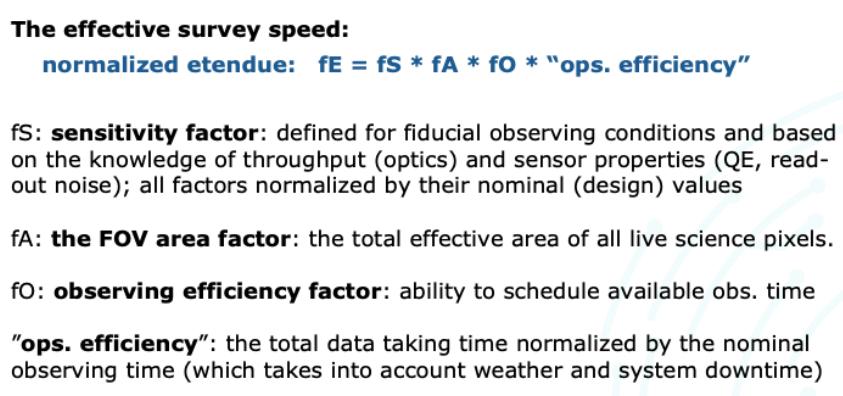
\includegraphics[width=0.75\linewidth]{fE.png}
\caption{Dimensionless survey efficiency factor, fE. Only ops efficiency is not known precisely at this time by data or design. The ComCam run will allow a specific determination of fE as we roll into LSSTCam commissioning. fE will be fully updated by as built system performance and ops. efficiency by the end of science validation.}
\label{fE}
\end{figure}

All f factors are dimensionless and normalized by the corresponding SRD design values. They can be “traded against each other” as “time”.
For example, deterioration in the mirror reflectivity can be easily translated to factor fS, and traded against time (e.g. time lost to recoating, the system “efficiency”), or against loss of sensor area (fA).
The key point is that it is possible to define a simple measurable quantity (fE) that is an excellent numerical approximation for “LSST science goals”. Thus, we can think of the effective speed of executing the LSST (in units of the nominal speed) in terms of recognizable elements: fE ~ ”eff area” * “eff FOV” * “cadence” * “downtime”

In Figure~\ref{speed}, we show the current state of our understanding of the image quality and survey speed.

\begin{figure}[t]
  \centering
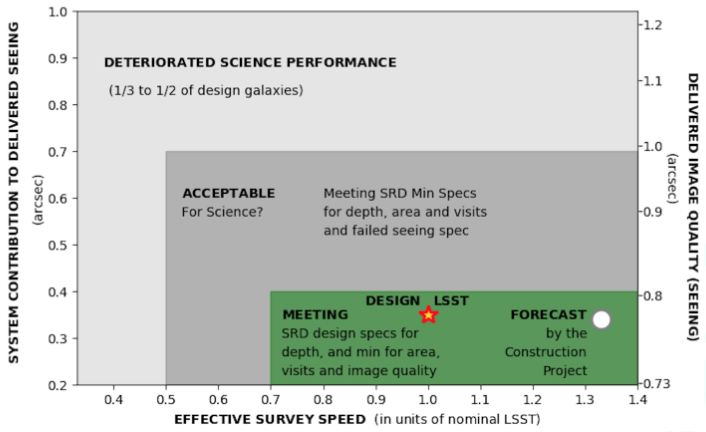
\includegraphics[width=0.85\linewidth]{speed.png}
\caption{Image quality versus effective survey speed, fE. The system contribution to the image quality is shown on the left vertical axis and the delivered image quality including the atmosphere (added in quadrature) is on the right. The LSST design is accomplished with nominal speed 1.0 and system IQ of 0.35$''$ in this diagram. Based on known subsystem performance and design, the current forecast shows the LSST will be accomplished with significant margin. Any final margin will be used to reassess the survey strategy given by \cite{PSTN-056}.}
\label{speed}
\end{figure}

There are three regions in the diagram. Clearly we want to be in the green shaded region and to the lower right in the space. The current understanding og the system as verified through subsystem verification or from the design and median seeing from the free atmosphere (0.7$''$) suggests we are in good shape. Experience with ComCam in late 2024 suggests we should be able to reach high ops efficiency. This will be quantified in the upcoming LSSTCam commissioning period.  



\section{Criteria to begin the LSST}

Armed with an understanding of the {\it as--built} system performance as outlined above and the Operations team readiness, we will use a set of objective criteria to gate the start of the LSST. These criteria will be concise and easily understandable so that the community of scientists, Rubin staff and other stakeholders counting on Rubin and the survey can have confidence the Observatory is on track.

The criteria articulated below are meant only to provide gating guidance signifying the survey start. There will be key processes within the overall system, including data management and processing where further work for improvements are required or desired after handover (beyond the construction project requirements). Unless these would prevent the acquisition and saving of science quality data, thereby delaying the survey start, they are not discussed or enumerated here.  These and other criteria (TBD) will be used to gauge and monitor the overall performance of the Observatory and progress towards the 10--year survey objectives going forward, with nominal $T_0$ defined by when start criteria described herein are met.

The initial set of criteria developed by Operations team were discussed with the Science Advisory Committee and community at the 2024 Rubin Community Workshop. These criteria have evolved since that meeting and are presented here in Table~\ref{tab:criteria}.

\begin{table}[]
\renewcommand{\arraystretch}{2}
\small
\centering
\caption{Survey Start Criteria}\label{tab:criteria}
\begin{longtable}{|p{0.25in}|p{1in}|p{4in}|p{1.0in}|}
\hline
Item & Criterion & Description& Status \\
\hline \hline

1 & \makecell[l]{LSSTCam\\ Maintenance} & Before the completion of SV, it is understood whether or not off TMA Camera maintenance will be needed within the first year of Operations.& \makecell[l]{\\No off TMA \\maintenance\\ required.\\}  \\\hline  

2 & SRD & All science requirements that can be verified with SV data are verified or expected to be verified within 3 months of completion of SV. & Check status at CCR3 \\\hline

3 & Dome & The dome environment is not limiting typical performance. &\makecell[l]{\\Not controlled \\until after \\Handover\\}\\\hline

4 & Calibration & All necessary calibration data products are available at the time any LSST data are obtained or can be obtained after the fact without invalidating the observed data for inclusion in the LSST. & Check status at CCR3 \\\hline

5 & sDIQ & The ``System'' contribution to the measured Delivered Image Quality is better than or equal to 0.45$\arcsec$ & \makecell[l]{\\Currently 0.6$\arcsec$ \\system \\contribution\\}\\\hline

6 & sDIQ Uniformity& The ``System'' contribution to the measured Delivered Image Quality can vary over the field of view such that 10$\%$ or less of the FOV has a system contribution of up to 0.52$\arcsec$ (see LSST system specifications LSR-REQ-0008.  & \makecell[l]{\\Currently\\ not meeting \\for typical\\images\\}\\\hline

7 & Ellipticity & Ellipticity for a single image will typically be as specified in the LSST system requirements as  LSR-REQ-0092. This is $\leq$ 0.04 with 5$\%$ or fewer outliers beyond 0.07.& \makecell[l]{\\In SV, \\typically not \\meeting\\}\\\hline

8 & Normalized \'{E}tendue (\it{eF}) & Survey Speed  is $>$ 0.7. & Currently 0.68 \\

\hline
\end{longtable}
\end{table}

\newpage 

\begin{table}[]
\renewcommand{\arraystretch}{2}
\small
\centering
\caption*{Survey Start Criteria Continued}
\begin{longtable}{|p{0.25in}|p{1in}|p{4in}|p{1.0in}|}
\hline
Item & Criterion & Description& Status \\
\hline \hline

10 & LHN ready & The Long Haul Network will be working reliably and not be a limiting factor in Alert Production & LHN is ready and not limiting Alert Production\\\hline

11 & DM ready& The data management system is ready & DM is ready \\\hline

12 & Early Science & DP2 observations are completed as planned \citep{RTN-011}.& \makecell[l]{\\SV is complete; \\a report will be \\delivered by \\October.\\} \\

\hline
\end{longtable}
\end{table}

The initial boundary conditions for determining the start criteria are that the construction project has successfully accomplished its own Construction Completeness Criteria (\cite{SITCOMTN-005}) and has passed the third Construction Completeness Review (CCR3).  Successful completion of CCR3 means NSF and DOE have accepted the system as the one that was intended to be built and will operate to conduct the 10-year LSST science program.  

The survey start criteria cover a range of contexts.  The criteria are not meant to be comprehensive with respect to gauging and monitoring LSST's scientific progress and success. They are intended to serve as a guide for the confident commencement of the survey -- effectively establishing what will be referred to as LSST T$_0$.  Most of the defined criteria look to be well in hand based on what we know about commissioning progress and system performance as reported at CCR2/ORR1.  Of the 8 criteria enumerated we have identified what we call ``The Big 3,'' : the ``system'' contribution to the Delivered Image Quality (sDIQ) with two primary contributors -- (1) the interior dome environment plus (2) the hardware system (optics, tracking etc.), and (3) the effective survey speed or Normalized \'{E}tendue. 

Looking at the criteria in Table~\ref{tab:criteria}, Item 1 is already met. We do not expect to have to remove the camera for maintenance before we begin the survey. Item 2 is needed to ensure some key aspects of the system don't need verification before we embark on the LSST. Some long term SRD requirements need a significant amount of data to finally validate. But we can be assured data being taken are going to be valid for the LSST if the requirements that can be validated with SV data have been validated. This will be confirmed at CCR3. The calibration system (item 4)  is in the advanced stages of validation. By CCR3, we can be assured no outstanding calibration needs will limit the taking of images for the LSST. 

For item 9, the Survey Cadence Optimization Committee has delivered to the Operations Directorate one (or more) proposed survey cadence algorithms to be implemented using the Feature Based Scheduler.  The scientific merits and technical feasibility of the proposed algorithm(s) will have been reviewed (If more than one proposal is provided a selection is made).  This selection will be the core algorithm adopted through LSST observations leading to the first data release DR1.  Remaining minor adjustments to the adopted algorithms are expected to be made as needed.  The adopted cadence algorithm has been verified with simulations using as--built performance, by on-sky operations using the Feature Based Scheduler.  SV data taking is complete, so we know the content of DP2 from SV (item 12) and only now need to decide whether or not any significant augmentations are critical for community preparation prior to data release 1 \citep[DR1; see][]{RTN-011}. 

For items 10 and 11, our SV experience shows these are ready, or in any case, sufficient for starting the survey. The Long Haul Network (LHN) has been working reliably and will not limit alert production. DM has produced, from end to end, Data Preview 1 \citep[DP1; see][]{RTN-095}. There is continuous development to be done, but nothing to stop the start of the survey.  

This leaves ``The Big 3'' -- the system contribution to the Delivered Image Quality (optics + dome environment) and Normalized \'{E}tendue.

\subsection{Delivered Image Quality (DIQ)}

The single most important gain needed to get to the LSST start is clearly the typical DIQ.  We will not start the LSST until the sustained performance of the system contribution to DIQ is $\le$ 0.45$\arcsec$.  This criteria is the combination of both the telescope + LSSTCam optics and the degradations caused from any thermal non-equilibrium. Currently the very least the active optics contributes to the system has been measured at 0.33$\arcsec$.  The target for the active optics contribution is 0.25$\arcsec$ indicating there is room for improvement.  In addition to the active optics contribution, much of the remaining improvement needed to meet the system DIQ start criterion will come from system thermal control (mostly the dome environment).

Improving the system contribution to the DIQ requires continued effort on the control of optics and the dome environment. Putting this together with the criteria above results in the region of the performance diagram we can use to gate starting the LSST as depicted in Figure~\ref{speed3}. The survey can begin once the system contribution to DIQ is 0.45$\arcsec$ or less and the effective survey speed is 1.01 or better (see Table~\ref{tab:factors} and assume System Availability is 75$\%$).

Equally important for the scientific value of the images is that the typical LSST images meet the requirements for uniformity across the field of view and ellipticity for bright isolated stars. These are given in Table~\ref{tab:criteria}. For uniformity to start the survey, we identify the value of the allowed contribution in the worst quartile of the overall seeing profile given in the SRD. This is 0.52$\arcsec$. 

\subsection{Dome Environmental Control}
The dome will be the last major subsystem to be completed. Indeed it will not be done until mid 2026. The critical aspects that are needed are: to install, provide control for, and optimize the actuators for the dome louvers and the installation of the HVAC ductwork used for daytime thermal conditioning of the dome interior. There are 40 louvers, and some large fraction need to be operable (open at fractions consistent with telemetry in real time for temperatures and wind). The first actuators are installed now and one louver has been opened at night. Still more will need to be brought on line after the handover to meeting the system image quality criterion (we currently expect 12 will be operable after handover). If the louvers limit us to worse than typical system DIQ performance, we won't be able to start the LSST until they are largely deployed and in routine operation. 

There are large ducts that will provide conditioned air distribution supplied by the main air handlers inside the facility. This system is designed to pre-condition the internal dome environment during daytime hours to minimize thermal discontinuities at the start of each night caused by diurnal heating.  This system is designed improve our ability to maintain the enclosure at closer to the anticipated mean nighttime temperature during the (earlier) day time. Maintaining thermal equilibrium in the environment in and around the telescope is critical to optimum DIQ during the night. The ducts are necessary but not sufficient. We will also need to gain experience in forecasting the coming night's temperature to be able to use the air conditioning effectively (i.e. to set the system to hit the right target). 

Further use of available temperature sensors on the telescope and in the dome will help on going analyses aimed at improving the AOS and thermal control of the optics in real time. 

The total contribution to DIQ from the dome environment is modest. Including all sources of turbulence generated by the facility, the budget (i.e residual contribution after control) to contribute to the DIQ is only 0.09$\arcsec$. Clearly all systems for controlling these contributions need to be working well and reliably. The observatory will need to rely on the ability to characterize parts of the DIQ coming from this environment. Thus we will prioritize reliable operation and calibration of our DIMM, in-dome seeing monitors, as well as the atmospheric profiler on Cerro Pach\'{o}n, RINGSS.  

\subsection{Normalized \'{E}tendue}
Much of the effective speed (Normalized  \'{E}tendue) is already demonstrated to be sufficient to start the LSST, The field of view factor, fA, is excellent and stable. The sensitivity factor, fS, is also very good. This factor has the potential to help overall performance because of its dependence on delivered image quality. Getting the system contribution from 0.6 to 0.4 (coupled with site free air atmospheric seeing of 0.7$\arcsec$) would raise fS from 0.94 to 1.3. Apart from this, all the optics are delivered as is the focal plane. The performance of all these components is excellent and can be maintained. The observing efficiency or fO is also in good shape. The telescope dynamic performance (slew speed, acceleration, and jerk) is sufficient for the LSST planned cadence. 

The TMA is capable of accelerating more than we currently operate it. Higher acceleration requires improvements in the control of dynamic loads on the M1M3 glass via force actuators. However the current performance with glass is captured in the scheduler simulator and is only a modest hit to overall survey speed. We will continue to work on improved dynamic control even as we operate for LSST. Slew and settle performance are well understood and adequate. Modest gains on fO are forecast for the rest of SV and early operations. We expect the current value to go from 0.97 to 1.05. 

This leaves the System Availability, Current performance of 0.75 needs to be improved. Doing only science like observations we have reached 85$\%$ at times. We need to continue to improve on procedures and reliability of systems throughout the summit facility as we go forward. This means training for faster troubleshooting and fault recovery, making communications on the telescope system bus more reliable, improving reliability of telescope, dome, and camera functions. These have all seen marked progress as expected throughout system integration, test, and commissioning. We will assume current performance of 75$\%$ conservatively. 

Using the combined SRD minimum specifications the lowest Normalized \'{E}tendue allowed is 0.7. This level is nearly in hand; see Table~\ref{tab:factors} and the ''Sustained Performance values''. We will start the LSST consistent with System Availability of 75$\%$ which leads to fE $=$ 1.01 using the Needed to Start LSST column f factors in Table~\ref{tab:factors}. However, the actual value will be better given that we expect the System Availability to improve significantly. 

\begin{figure}[t]
\centering
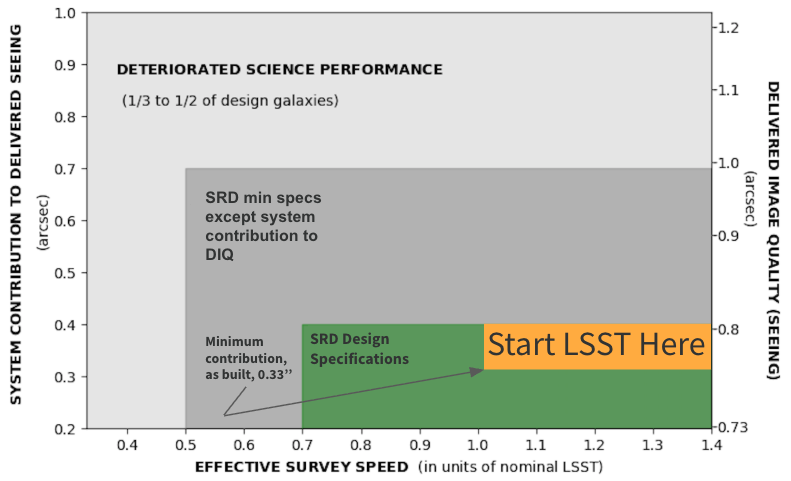
\includegraphics[width=0.85\linewidth]{speed3.png}
\caption{Image quality versus effective survey speed or Normalized \'{E}tendue. The large orange rectangle represents the region in this space within which we can confidently start the LSST while working to maintain and improve performance.}
\label{speed3}
\end{figure}

\newpage

\section{Schedule}{\label{secSched}}

The Project and Operations teams will complete several reviews as described below in order to closeout the construction phase, handover to Operations, and demonstrate readiness to begin the LSST. The first of these, Construction Completeness Review (CCR) 1, was held in October, 2024. CCR2 took place in July, 2025. Concurrent to CCR2, the Operations team went through the Operations Readiness Review (ORR) 1. Both reviews were run in parallel with the same NSF--DOE review panel convened to review and report out for the Observatory as a whole. A modest set of recommendations were made and Construction and Operations are addressing them. 

Construction Closeout and Operations Readiness Reviews:

\begin{itemize}
\item CCR1 -- readiness for the start of on-sky commissioning, as exemplified by substantial completion and integration of subsystems, and evidenced by direct measurement of the optical throughput of the integrated system

\item CCR2 -- capability to support LSST science goals, as exemplified by the System First Light technical milestone, and evidenced by delivered single-visit image quality (including active control of optics)

\item CCR3 -- reliability to initiate the LSST survey, as exemplified by the Science Validation Surveys, and evidenced by the readiness of Rubin Observatory Operations to accept the as-built Observatory

\item CCR4 -- closeout of the Construction project, as exemplified by service of scientifically validated survey-scale data products as part of the Operations Early Science Program, and evidenced by completed scope of system-level requirement verification, reporting, and final accounting
\end{itemize}

As of September 2025, the science validation phase of Construction is nearly complete. SV and system optimization will run through September 22. The facility will then shut down until October 24 to complete the remaining large integration activities that are required before starting regular operations. It is known that a number of activities will continue in operations managed by the construction project. These activities are captured in the "punch list". It is expected approximately 10 FTE of effort in FY26 going through at least June will be required to finish the punch list. 

CCR3/ORR2 will be held in October at the end of the observatory shut down. The combined review will be held with Observatory, partner, and agency staff. No review panel will be present. The team will present the status of the observatory following SV and the shutdown activity, the plans for the punch list, and the plans for early operations regarding continued optimization and readiness to start the LSST.

Following CCR3/ORR2 and the concurrent "Handover", the Operations team will begin to regularly run the system, taking responsibility for the observatory on October 25th. The priority for the Operations team is to drive the system to the state captured by the criteria in this document and start the LSST. Figure~\ref{sched} shows the current milestones for the Project and Operations. The period after CCR3/ORR2 is uncertain, but likely will involve continued pre--survey optimization. 

\begin{figure}%[]
  \centering
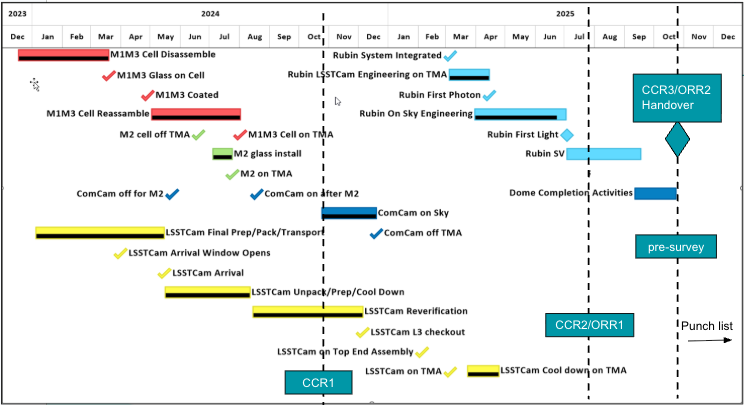
\includegraphics[width=0.95\linewidth]{sched.png}
\caption{Rubin Observatory Schedule as of September 01, 2025. Formal completeness reviews including operations readiness are shown in the Figure and described above. Handover to the Operations is set for October 25, 2025 and pre-survey optimization will continue until the performance criteria described in this document are met for starting the LSST. In parallel, some activities and work by the Construction team will continue in FY26. Some of these activities will positively impact on sky performance. }
\label{sched}
\end{figure}

\newpage


%\appendix

% Include all the relevant bib files.
% https://lsst-texmf.lsst.io/lsstdoc.html#bibliographies

\section{References} \label{sec:bib}

\renewcommand{\refname}{} % Suppress default Bibliography section
\bibliography{local,lsst,lsst-dm,refs_ads,refs,books}

% Make sure lsst-texmf/bin/generateAcronyms.py is in your path
\section{Acronyms} \label{sec:acronyms}
\addtocounter{table}{-1}
\begin{longtable}{p{0.145\textwidth}p{0.8\textwidth}}\hline
\textbf{Acronym} & \textbf{Description}  \\\hline

AOS & Active Optics System \\\hline
AURA & Association of Universities for Research in Astronomy \\\hline
CCR & Construction Completeness Review \\\hline
CCR1 & Construction Completeness Review 1 \\\hline
CCR2 & Construction Completeness Review 2 \\\hline
CCR3 & Construction Completeness Review 3 \\\hline
CCR4 & Construction Completeness Review 4 \\\hline
DIMM & Differential Image Motion Monitor \\\hline
DIQ & Delivered Image Quality \\\hline
DOE & Department of Energy \\\hline
DP2 & Data Preview 2 \\\hline
DR1 & Data Release 1 \\\hline
FOV & field of view \\\hline
FTE & Full-Time Equivalent \\\hline
FWHM & Full Width at Half-Maximum \\\hline
FY26 & Fiscal Year 2026 \\\hline
FoV & Field of View (also denoted FOV) \\\hline
HVAC & Heating, Ventilation, and Air Conditioning \\\hline
LPM & LSST Project Management (Document Handle) \\\hline
LSE & LSST Systems Engineering (Document Handle) \\\hline
LSR & LSST System Requirements; LSE-29 \\\hline
LSST & Legacy Survey of Space and Time (formerly Large Synoptic Survey Telescope) \\\hline
M1M3 & Primary Mirror Tertiary Mirror \\\hline
M2 & Secondary Mirror \\\hline
MREFC & Major Research Equipment and Facility Construction \\\hline
NOIRLab & NSF's National Optical-Infrared Astronomy Research Laboratory; \url{https://noirlab.edu} \\\hline
NSF & National Science Foundation \\\hline
OPS & Operations \\\hline
ORR & Operations Readiness Review \\\hline
ORR1 & Operations Readiness Review 1 \\\hline
ORR2 & Operations Readiness Review 2 \\\hline
OSS & Observatory System Specifications; LSE-30 \\\hline
PSF & Point Spread Function \\\hline
PSTN & Project Science Technical Note \\\hline
QE & quantum efficiency \\\hline
RDO & Rubin Directors Office \\\hline
RINGSS &  \\\hline
RTN & Rubin Technical Note \\\hline
SA & System and Services Acquisition \\\hline
SCOC & Survey Cadence Optimization Committee \\\hline
SLAC & SLAC National Accelerator Laboratory \\\hline
SRD & LSST Science Requirements; LPM-17 \\\hline
SV & Science Validation \\\hline
TBD & To Be Defined (Determined) \\\hline
TMA & Telescope Mount Assembly \\\hline
US & United States \\\hline
USDF & United States Data Facility \\\hline
\end{longtable}

% If you want glossary uncomment below -- comment out the two lines above
%\printglossaries

\end{document}
